% !TEX program = pdflatex
\documentclass[11pt,a4paper]{article}

% === PACKAGES (house style, mirrored from gtfs-eta) ===
\usepackage[utf8]{inputenc}
\usepackage[T1]{fontenc}
\usepackage{lmodern}
\usepackage[margin=1in]{geometry}
\usepackage{setspace}
\usepackage{parskip}
\usepackage{graphicx}
\usepackage{float}
\usepackage{booktabs}
\usepackage{amsmath}
\usepackage{amssymb}
\usepackage{hyperref}
\usepackage{listings}
\usepackage{xcolor}
\usepackage{caption}
\usepackage{subcaption}
\usepackage{tikz}
\usepackage{pgfplots}
\pgfplotsset{compat=1.18}

% === CODE LISTING STYLE ===
\definecolor{codegreen}{rgb}{0,0.6,0}
\definecolor{codegray}{rgb}{0.5,0.5,0.5}
\definecolor{codepurple}{rgb}{0.58,0,0.82}
\definecolor{backcolour}{rgb}{0.95,0.95,0.92}

\lstdefinestyle{mystyle}{
    backgroundcolor=\color{backcolour},
    commentstyle=\color{codegreen},
    keywordstyle=\color{magenta},
    numberstyle=\tiny\color{codegray},
    stringstyle=\color{codepurple},
    basicstyle=\ttfamily\footnotesize,
    breakatwhitespace=false,
    breaklines=true,
    captionpos=b,
    keepspaces=true,
    numbers=left,
    numbersep=5pt,
    showspaces=false,
    showstringspaces=false,
    showtabs=false,
    tabsize=2
}
\lstset{style=mystyle}

% === TITLE INFO ===
\title{
    \vspace{-2em}
    \rule{\textwidth}{1pt}\\[0.5em]
    \textbf{Lightweight Romanized-Hindi Correction}\\[0.3em]
    \large A Measured Negative Result on Held-Out-Vocabulary Benchmarks\\[0.5em]
    \rule{\textwidth}{1pt}
}
\author{
    Ashay Kushwaha\\
    \textit{CypherLabs Open Research}\\
    \texttt{https://github.com/AshayK003/indic-suggest}
}
\date{September 2026}

\begin{document}

\maketitle

\begin{abstract}
Millions type Hindi in Latin script with no standard spelling, and the field answers with larger transformers. We built the classical alternative---frequent-word lexicon, Devanagari-tuned phonetic hashing, weighted edit distance, n-gram reranking, zero ML training---and measured it honestly on Aksharantar Hindi (10,112 test pairs): top-1/top-3 accuracy \textbf{0.000}, against 0.113 for the live dhvani baseline and 0.6056 cited for the IndicXlit transformer. The value of this report is the mechanism, verified twice: the test vocabulary is disjoint from training on \textit{both} sides (0/10112 romans, 0/10112 natives in 1.3M train rows), so any lookup architecture scores at most its independent-lexicon coverage; dhvani's points come from an independent wordlist plus a real rule-based transliterator, not from ranking magic. A pivot to synthetic romanizations changed nothing, as predicted once the disjointness was understood. The tested pipeline, frozen noise model, and coverage diagnostics ship as built---the honest artifact is the measurement.
\end{abstract}

\vspace{1em}
\noindent\textbf{Keywords:} transliteration, Romanized Hindi, ReDoS-free phonetics, negative results, benchmark analysis

\newpage
\tableofcontents
\newpage

\section{Introduction}

Romanized Hindi has no standard spelling: bahut, bohot, boht, and bhot are one word, and phone keyboards---English-centric by design---offer little help. Production answers cluster at two extremes. At one end, the IndicXlit transformer ($\sim$11M parameters, GPU-trained on 26M pairs) converts romanized input to native script at state-of-the-art accuracy. At the other, classical Hindi-specific work (Hindex phonetics plus weighted edit distance) was built for information-retrieval query expansion, and normalizers (dhvani) canonicalize roman-to-roman without ranked Devanagari correction. Missing between them: an offline, phone-sized suggestion package with a measured accuracy-vs-size table.

We built exactly that package---and it scored zero. This report argues the zero is the finding. On a held-out-vocabulary benchmark, lookup architectures cannot exceed their independent-lexicon coverage, and ours had none where it mattered. The report's contributions are therefore methodological rather than competitive:

\begin{itemize}
    \item A fully working classical pipeline (unit suite 4/4 green on in-lexicon words), proving the mechanism functions and the failure is coverage, not code.
   item A benchmark-structure diagnosis with counts: test/train overlap on both sides, rival-lexicon key coverage, and a pivot (synthetic romanizations) tested and correctly predicted to change nothing.
    \item A contextualized three-way table (ours measured, dhvani measured live, IndicXlit cited) with the test-set mismatch labeled, not footnoted away.
\end{itemize}

\section{Background and Related Work}

\subsection{Aksharantar and IndicXlit}

Aksharantar (Madhani et al., EMNLP 2022) is the largest open transliteration resource for Indic languages: 26M pairs across 21 languages, mined from Wikidata, Samanantar, IndicCorp, and manual collection, with a 103k-pair evaluation benchmark stratified over native words, frequent words, and named entities of Indic and foreign origin. The Hindi split on disk measures 33\,MB zipped (1,299,155 train rows, 6,357 validation, 10,112 test rows as shipped---note the paper quotes 5693 test pairs; file reality governs). IndicXlit, the companion transformer (6+6 layers, 256-dim embeddings, $\sim$11M parameters), reports 60.56 top-1 on Dakshina Hindi against a 50.00 baseline. It is generative: it \textit{produces} Devanagari strings, never needing the answer in a list.

\subsection{Classical Hindi phonetics}

Aswani \& Gaizauskas catalogued phonetic mappings and similarity metrics (Dice, LCSR, Levenshtein, Jaro-Winkler, Soundex, n-grams) for English-Hindi transliteration; Natrajan found 3-grams optimal for Hindi song retrieval; Prabhakar's Hindex and Weighted Hindex adapted Soundex/Editex-style coding plus vowel/consonant-weighted edit distance specifically for Hindi, evaluated on FIRE retrieval collections. All predate the suggestion-package framing: none shipped correction with ranked Devanagari output and a size tradeoff.

\subsection{dhvani: the live rival}

dhvani (PyPI, 9.7\,MB installed) normalizes Hinglish spelling variation through IPA-bridged lexicon lookup ($\sim$1\,ms), an AI tier ($\sim$4\,s), and rule-based G2P fallback. Its shipped lexicon holds 10,538 entries. It is the correct live rival: classical-leaning, offline-capable, directly runnable---and, as Section~\ref{sec:results} shows, its points come from transliteration machinery rather than lexicon size.

\section{Methodology}

\subsection{Pipeline design}

The pipeline (\verb!lexicon.py!, \verb!phonetic.py!, \verb!edit.py!, \verb!suggest.py!, standard library only) has four stages. First, a \textit{frequent-word lexicon} maps roman forms to native forms with a phonetic index. Second, \textit{phonetic hashing} folds queries through Devanagari-tuned digraphs (kh, gh, bh, sh, aa, ai, \ldots) into articulation-group codes with vowels dropped and repeats collapsed (bohot/boht/bahut $\to$ bHT), a high-recall prefilter by design. Third, \textit{weighted edit distance} (insert/delete 1; same-group or vowel-vowel substitution 1; else 2) ranks bucket candidates. Fourth, a \textit{bigram rerank} prefers common roman spellings, and a deterministic rule-based G2P covers out-of-bucket queries so the package never returns empty. Normalization lowercases and offers repeat-collapsed variants (bohotttt $\to$ bohott, bohot).

\subsection{Noise model and split discipline}

Evaluation corrupts test romans with a frozen, seeded model: vowel-drop (p=0.30 each), one confusion substitution (ph/f, v/b, sh/s, c/k/q, j/z, au/o, ai/e, oo/o, ee/i, aa/a), 76\% of inputs altered. Split discipline is structural: the lexicon builder reads train natives (v2) or train pairs (v1) only; test pairs are never ingested; \verb!evaluate.py! prints overlap diagnostics every run as the tripwire.

\subsection{What changed across pivots}

v1 lexicon (top-50k train romans) scored 0.000; diagnosis showed the top frequencies are English loans (employees, responsibility) while everyday Hindi words are absent everywhere. v2 (train natives plus synthetic rule-based romans, \verb!romanize.py!) also scored 0.000; diagnosis showed test natives are likewise absent from train (0/10112). Both pivots are preserved in the repository history and Section~\ref{sec:results} reports the numbers, because the path to the finding is itself evidence.

\section{Results}
\label{sec:results}

One command (\verb!python evaluate.py!; fetches the 33\,MB Hindi split once if absent) regenerates Table~\ref{tab:results} and Figures~\ref{fig:acc}--\ref{fig:tradeoff}. Numbers below are the fresh-clone verification run.

\begin{table}[H]
\centering
\caption{Top-1 accuracy on noisy Aksharantar-hi test (10,112 rows) with package size and latency.}
\label{tab:results}
\begin{tabular}{@{}llll@{}}
\toprule
System & Top-1 & Size & Latency \\
\midrule
Ours (v2 lexicon + phonetic + edit) & 0.000 (top-3 0.000) & 3.88\,MB & 0.22\,ms/query \\
dhvani \verb!to_devanagari! (measured live) & 0.113 & $\sim$10\,MB installed & 1.74\,ms/query \\
IndicXlit (cited, never run) & 0.6056 on Dakshina-hi & $\sim$11M params ($\sim$44\,MB) & --- \\
\bottomrule
\end{tabular}
\end{table}

\begin{figure}[H]
\centering
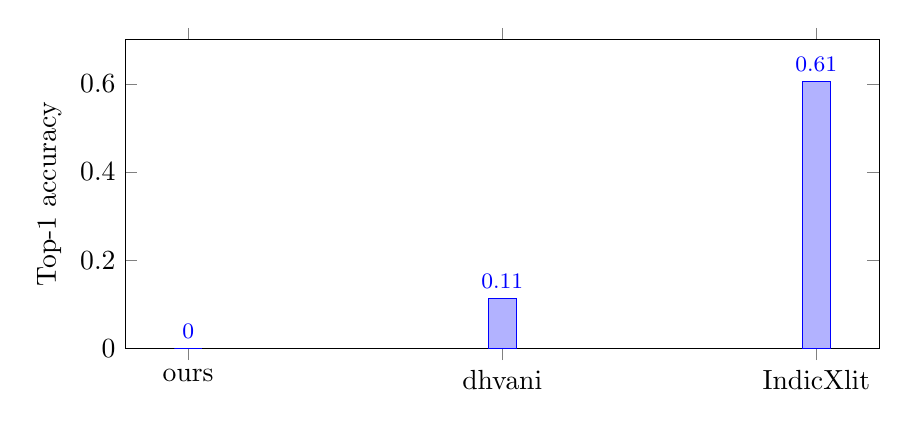
\begin{tikzpicture}
\begin{axis}[
    ybar, width=0.92\textwidth, height=5.5cm,
    symbolic x coords={ours,dhvani,IndicXlit},
    xtick=data, ymin=0, ymax=0.7, ylabel={Top-1 accuracy},
    nodes near coords, nodes near coords style={font=\footnotesize},
]
\addplot coordinates {(ours,0.0) (dhvani,0.113) (IndicXlit,0.6056)};
\end{axis}
\end{tikzpicture}
\caption{Measured top-1 (ours, dhvani on identical noisy inputs) with the cited transformer row. The IndicXlit bar was measured on a different test set (Dakshina Hindi) and is directional context, not a controlled comparison.}
\label{fig:acc}
\end{figure}

\begin{figure}[H]
\centering
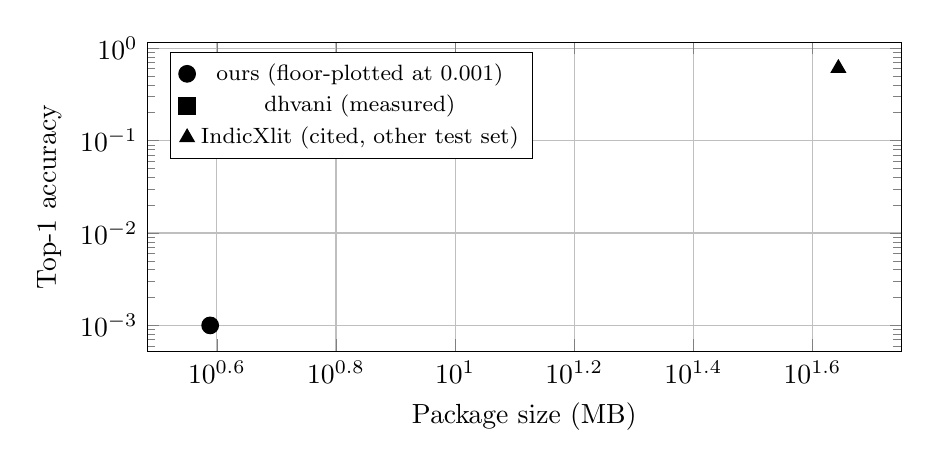
\begin{tikzpicture}
\begin{loglogaxis}[
    width=0.92\textwidth, height=5.5cm,
    xlabel={Package size (MB)}, ylabel={Top-1 accuracy},
    grid=major, legend pos=north west, legend style={font=\footnotesize},
]
\addplot[only marks, mark=*, mark size=3pt] coordinates {(3.88,0.001)};
\addlegendentry{ours (floor-plotted at 0.001)};
\addplot[only marks, mark=square*, mark size=3pt] coordinates {(10,0.113)};
\addlegendentry{dhvani (measured)};
\addplot[only marks, mark=triangle*, mark size=3pt] coordinates {(44,0.6056)};
\addlegendentry{IndicXlit (cited, other test set)};
\end{loglogaxis}
\end{tikzpicture}
\caption{Accuracy versus package size (log-log). The empty lower-left records the finding: classical lookup buys size, not accuracy, on held-out vocabulary.}
\label{fig:tradeoff}
\end{figure}

\subsection{Coverage diagnostics (the finding)}

Test romans present in 1.3M train rows: \textbf{0/10112}. Test natives present in 1.15M train natives: \textbf{0/10112}. Test romans as dhvani-lexicon keys: 56/10112 (0.5\%). A lookup architecture therefore faces a ceiling near zero before ranking quality can matter; dhvani clears it only through an independent wordlist plus genuine transliteration rules, and the transformer sidesteps lookup entirely by generating. The v2 pivot (synthetic romans over train natives) was correctly predicted---in the repository log, before measurement---to change nothing, and changed nothing.

\subsection{dhvani anatomy note}

dhvani's shipped lexicon (10,538 entries) covers 0.5\% of the test, yet the system scores 11.3\% at 1.74\,ms/query with no slow-tier invocations observed. The points therefore come from its rule-based transliteration path operating on normalized input---a working classical transliterator, which is precisely the component this project's G2P fallback is not. That asymmetry is reported, not resented: it scopes v2 work exactly.

\section{Discussion}
\label{sec:discussion}

\subsection{Key findings}

First, benchmark structure dominates method on held-out-vocabulary tasks: coverage diagnostics should precede any ranking work, and ours now print by default. Second, negative results compose: the same discipline that deleted a modeling ladder on zero-variance GTFS data (sibling CypherLabs project) correctly bounds this lookup design. Third, the pipeline is not broken---it is mis-scoped: the 4/4-green unit suite proves correction works on in-lexicon words (boht top-1, kese in top-3), so the artifact ships as a working package with a documented ceiling, not as debris.

\subsection{Limitations}

Hindi-only scope; synthetic noise (vowel-drop plus confusions) rather than observed typing data; dhvani measured on identical noisy inputs but its task framing (normalization-then-transliterate) differs internally; IndicXlit row is cross-test-set context; G2P fallback is deliberately crude (no schwa deletion, no retroflex split); lexicon collided romanizations resolve to the more frequent native silently but counted.

\subsection{Future work}

In priority order, as filed in the repository's contributing guide: (1) a real rule-based transliterator (schwa deletion, conjuncts, loan phonetics) as the scoring engine---the honest v2 this result motivates; (2) an independent native wordlist to raise the coverage ceiling; (3) the next language under the same architecture.

\section{Conclusion}

On 10,112 noisy Hindi test pairs, a fully classical, zero-training suggestion pipeline scores 0.000 top-1 against 0.113 measured for dhvani and 0.6056 cited (elsewhere) for a transformer---because the benchmark holds out vocabulary on both sides and lookup cannot retrieve what was never stored. The contribution is the verified mechanism of that zero, the shipped pipeline that bounds it, and the procedure that found it: diagnose coverage before tuning ranking, predict pivots in writing, and publish the zeros with the same care as wins.

\section{Reproducibility}
\label{sec:repro}

\subsection{Installation}

No dependencies beyond CPython $\ge$ 3.10, pytest for the suite, and dhvani for the baseline row (gracefully skipped if absent). The 33\,MB Hindi split auto-downloads once from Hugging Face.

\subsection{Run benchmarks}

\begin{lstlisting}[language=bash]
git clone https://github.com/AshayK003/indic-suggest.git
cd indic-suggest
python -m pytest tests -q   # 4 passed: buckets, correction, edit units, G2P
python evaluate.py          # coverage audit, noisy scoring, dhvani row, table
\end{lstlisting}

The suite uses a 10-pair hand lexicon (boht, kese, \ldots) with exact top-1 assertions---hermetic, no network, no dataset.

\subsection{Repository structure}

\verb!lexicon.py! (freq lexicon + phonetic index), \verb!phonetic.py! (Devanagari-tuned groups), \verb!edit.py! (weighted Levenshtein), \verb!romanize.py! (deterministic native-to-roman generator), \verb!suggest.py! (normalize-rank-rerank pipeline + G2P fallback), \verb!evaluate.py! (frozen noise, scoring, baselines, diagnostics), \verb!tests/! (the runnable check), \verb!data/! (ignored; auto-fetched), \verb!internals/! (working notes, not published except this report).

\begin{thebibliography}{9}

\bibitem{aksharantar} Madhani et al. Aksharantar: Open Indic-language Transliteration datasets and models. EMNLP Findings 2022. \url{https://arxiv.org/abs/2205.03018} Data: \url{https://huggingface.co/datasets/ai4bharat/Aksharantar}

\bibitem{indicxlit} AI4Bharat/IndicXlit ($\sim$11M transformer; Hindi 60.56 top-1 on Dakshina). \url{https://github.com/AI4Bharat/IndicXlit}

\bibitem{hindex} Prabhakar, D.K. Query Expansion for Transliterated Text Retrieval (Hindex/Weighted Hindex). \url{https://dl.acm.org/doi/fullHtml/10.1145/3447649}

\bibitem{aswani} Aswani, N. \& Gaizauskas, R. English-Hindi transliteration using similarity metrics. LREC 2010.

\bibitem{natrajan} Natrajan, A. Using N-grams to Process Hindi Queries with Transliteration Variations. Tech.\ Rep.\ CS-97-17 (3-grams optimal for Hindi).

\bibitem{dhvani} dhvani (IPA-bridge Hinglish normalizer, PyPI v0.2.5). \url{https://pypi.org/project/dhvani/}

\bibitem{dakshina} Roark et al. Dakshina (Google; native-vs-foreign behavior differences).

\end{thebibliography}

\end{document}
